\documentclass{article}
\usepackage{listings}
\usepackage{tikz}
\usepackage[T1]{fontenc}
\usepackage{graphicx}
\usepackage{systeme}
\usepackage{fixltx2e}
\usepackage{subcaption}
\usepackage{multirow}
\usepackage{amsmath}
\usepackage{amssymb}
\let\emptyset\varnothing
\usepackage{commath}
\lstset{basicstyle=\ttfamily\footnotesize,breaklines=true}
\usepackage{float}

\title{Assignment  1\\ \vspace{0.2cm}

		COMP3670
}



\begin{document}
\setlength\parindent{0pt}
\maketitle
% \newpage
\vspace*{\fill}
    \begin{center}
    
        \textbf{name:}\author{Xuecheng Zhang}
        \\
        \textbf{UID:}u6284513
        
        \vspace{1.8cm}
        
        \date{5/8/2020}
    
    \end{center}
\vspace*{\fill}

\newpage

\textbf{Exercise 1 Solving Linear Systems (5+5 credits)}\\
Find the set S of all solutions x of the following inhomogenous linear systems Ax = b, where A and b are defined as follows. Write the solution space S in parametric form.\\

(a)
\begin{figure}[H]
  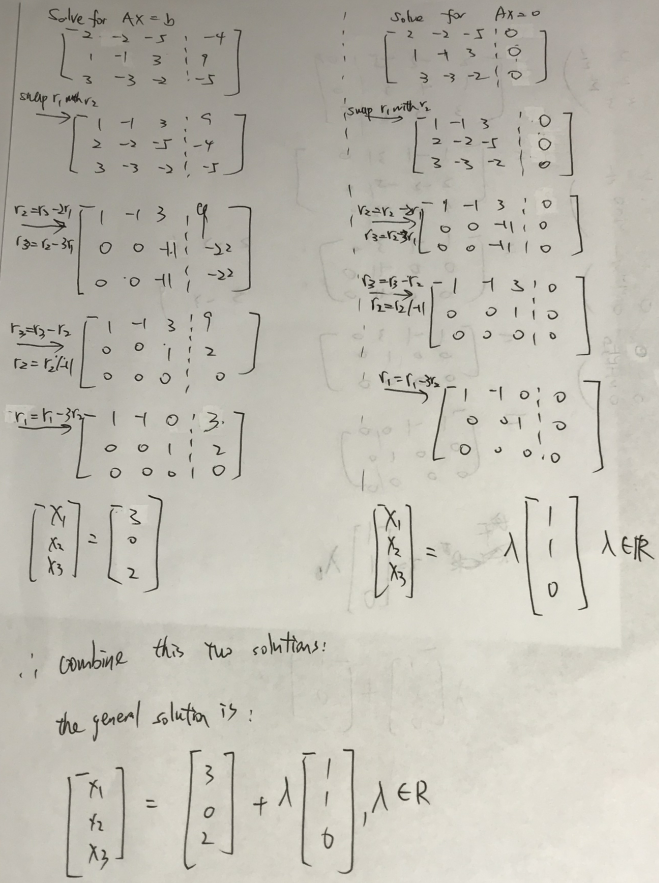
\includegraphics[width = \linewidth] {1a.JPG}
\end{figure}

\textbf{The solution Space S = $\Bigg\{\begin{pmatrix}
	3\\0\\2
\end{pmatrix} + \lambda \begin{pmatrix}
	1\\1\\0
\end{pmatrix} $, $\lambda \in \mathbb{R}\Bigg\}$\\}
(b)

\begin{figure}[H]
  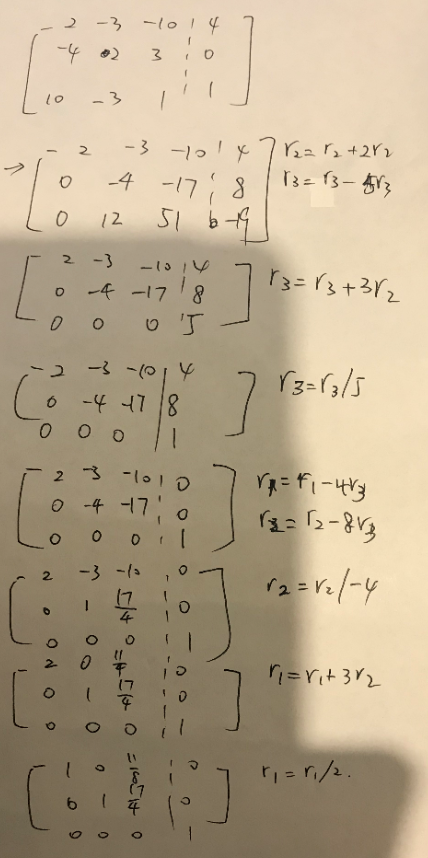
\includegraphics[width = 0.66\linewidth] {1b.JPG}
\end{figure}
\textbf{The system has no solutions and the Space S = $\emptyset$}\\


\textbf{Exercise 2 For what values of $\lambda$ does the inverse of the following matrix exist?}\\
When the inverse of matrix exists, the determinant of matrix cannot be 0.
\[
det =
\begin{vmatrix}
 \lambda & 1 & 2 & \\ 
 0 & 3 & 1\\
 1 & 1 & 1\\
\end{vmatrix} = 3\lambda+1-6-\lambda = 2\lambda -5 = 0
\]

If $\lambda$ $\neq$ $\frac{5}{2}$, the inverse of matrix exists.
\\\\
\textbf{Exercise 3 Which of the following sets are subspaces of $\mathbb{R}^{3}$. Prove your answer. (That is, if it is a subspace, you must demonstrate the subspace axioms are satisfied, and if it is not a subspace, you must show which axiom fails.)
}

(a) A = {(x, y, 1) : x, y, $\in$ R}\\
(b) B = {(x, y, z) : x + 4y - 3z = t}, where t is some real number. (Your answer may depend on the value of t.)\\
(c) C = {(x, y, z) : x $\geq$ 0, y $\geq$ 0, z $\geq$ 0}\\
(d) D = {(x, y, z) : x, y $\in$ $\mathbb{R}$, z $\in$ $\mathbb{Q}$}.\\

(a) It is not subspace of $\mathbb{R}^{3}$. Since 0 is not in A, A is not the subspace of $\mathbb{R}^{3}$ \\
(b) If t$\neq$0, then 0 $\notin$ B and it implies that B is not a subspace of $\mathbb{R}^{3}$.
\\ if t = 0, then 0 $\in$ B and B $\subseteq$ $\mathbb{R}^{3}$. \\
Also, assume $B_1$($x_1$,$y_1$,$z_1$) $\in$ B,  $B_2$($x_2$,$y_2$,$z_2$) $\in$ B, We get $x_1$ + 4$y_1$ - 3$z_1$ + $x_2$ + 4$y_2$ - 3$z_2$ = ($x_1$ + $x_2$) + 4($y_1$ + $y_2$) - 3( $z_1$ + $z_2$) $\in$ B, i.e. $B_1$ + $B_2$ $\in$ B\\
Assume $\lambda$ $\in$ $\mathbb{R}$, (X,Y,Z) $\in$ S and we can obtain that X + 4Y - 3Z = 0. 
$\lambda$ X + 4$\lambda$ Y - 3$\lambda$ Z = $\lambda$ ( X + 4Y - 3Z). i.e. $\lambda$(X,Y,Z) $\in$ S.\\
Therefore, we can conclude that when t$\neq$0, B is not a subspace of $\mathbb{R}^{3}$ and when t = 0, B is a subspace of $\mathbb{R}^{3}$.\\

(c) It is not subspace of $\mathbb{R}^{3}$. We assume that $C_1$ ($x_c$,$y_c$,$z_c$) $\in$ C, $C_2$ $\lambda$($x_c$,$y_c$,$z_c$) ($\lambda$ = -1). -$x_c$ $\leq$ 0; -$y_c$ $\leq$ 0;-$z_c$ $\leq$ 0; $C_2$ $\notin$ C. Therefore, C is not subspace of $\mathbb{R}^{3}$.\\


(d) It is not subspace of $\mathbb{R}^{3}$. Here is a counterexample, $D_1$ (2,3,4), $\lambda$ = $\sqrt{3}$, $D_2$ = $\lambda$ $D_1$ = (2$\sqrt{3}$,3$\sqrt{3}$,4$\sqrt{3}$), as 4$\sqrt{3}$ $\notin$ $\mathbb{Q}$. Therefore, D is not a subspace of $\mathbb{R}^{3}$.\\


\textbf{Exercise 4 Let v1, v2, v3 be vectors in $\mathbb{R}^{2}$. Prove that the set {v1, v2, v3} is linearly dependant.}\\
Assume v1,v2,v3 is linearly independent. From the definition of the basis of a vector space, v1,v2 can form a basis in $\mathbb{R}^{2}$ which means r3 can be written in terms of v1 and v2. It implies that v1,v2,v3 set is linearly dependent which draws the contradiction. Therefore, v1,v2,v3 is linearly dependent.\\

\textbf{Exercise 5}\\
(a) Is the following function $<.,.>$ defined for all x = $[x1, x2]^T$ $\in$  $\mathbb{R}^{2}$ and y = $[y_1,y_2]^T \in$ $R^{2}$ as <x,y> = $y_1(x_1 - x_2) + y_2(x_2 - x_1)$ \\
\textbf {It is not an inner mapping.} \\
For bilinear mapping: \\
\begin{gather}
\Omega(\lambda x + \phi y, z) =  z_1 (\lambda x_1 + \phi y_1 -\lambda x_2 - \phi y_2) + z_2(\lambda x_2 + \phi y_2 - \lambda x_1 - \phi y_1)\\
= \lambda (z_1x_1 - z_1x_2 + z_2x_2 - z_2x_1) + \phi(y_1z_1 - y_2z_1 + y_2z_2 - y_1z_2)\\
= \lambda\Omega(x,z) + \phi\Omega(y,z)
\end{gather}

\begin{gather}
\lambda \Omega (x,y) + \phi \Omega (x,z)=\lambda [y_1(x_1 - x_2) + y_2 (x_2 - x_1)] + \phi[z_1(x_1-x_2) + z_2(x_2-x_1)] \\
= (x_1 - x_2)(\lambda y_1 + \phi z_1) + (x_2 - x_1) (\lambda y_2 + \phi z_2)\\
= (\lambda y_1 + \phi z_1)(x_1 - x_2) + (\lambda y_2 + \phi z_2)(x_2 - x_1)\\
= \lambda(x,\lambda y + \phi z) 
\end{gather}
\textbf{It is satisfied with bilinear mapping.} \\

For symmetric axiom:\\
$<x,y> = y_1(x_1 - x_2) + y_2(x_2 - x_1) = x_1y_1 - x_2y_1 + x_2y_2 - x_1y_2$ \\
$<y,x> = x_1(y_1 - y_2) + x_2(y_2 - y_1) = x_1y_1 - x_1y_2 + x_2y_2 - x_2y_1$\\
Therefore $<x,y> = <y,x>$ is symmetric \\

\textbf{It is satisfied with symmertic axiom.}\\ 

For positive definite axiom:\\
$<x,x> = x_1(x_1 - x_2) + x_2(x_2 - x_1)$ = $x_1 ^2 - 2 x_1 x_2 + x_2^2 = (x_1 - x_2)^2 $\\if $x_1 = x_2$ then the formula equal to 0 instead of larger than 0.\\
Therefore, it is not positive definite matrix.\\

(b) Prove that <.,.> defined for all $x = [x_1, x_2]^T \in R^2$ and y = $[y_1,y_2]^T \in R^2$ as <x,y> = $x_1y_1-x_2y_2$ is not an inner product.\\

An inner product must satisfy positive definite axiom.\\ 
$\forall X \in R^2$ / ${0}, <x,x> = x_1y_1 - x_2y_2 = x_1^2 - x_2^2$ \\
if $x_1 < x_2 $ then $x_1^2 - x_2^2$ < 0. Therefore, it is not satisfied with positive definite axiom. i.e. it is not an inner product.\\


\textbf{Exercise 6}\\
(a) Prove that if x and y are linearly dependant vectors, then $|<x,y>| = ||x|| ||y||$\\
As x and y are linearly dependent vectors, then $c_1x + c_2y = 0, (c_1,c_2$  not all equal to 0). And we can derive that y = kx. \\
$|<x,y>| = |<x,kx>| = |k| |<x,x>| = |k| ||x||^{2}$\\
$||x|| ||y|| = ||x|| ||kx|| = |k| ||x||^{2}$\\
Therefore $|<x,y>| = ||x|| ||y||$\\
(b) Show that we can retrieve the inner product from the norm via the following expression:\\
$<x,y> = \frac{1}{2} (||x + y||^2 - ||x||^2 - ||y||^2)$\\

$\frac{1}{2} (<x+y,x+y> - <x,x> - <y,y>) $
\\ = $\frac{1}{2} (<x,x+y> + <y,x+y> - <x,x> - <y,y>)$\\
= $\frac{1}{2} (<x,x> + <x,y> + <y,x> + <y,y> - <x,x> - <y,y>) $\\
= $\frac{1}{2} * 2<x,y>$ = $<x,y>$ \\

Therefore the expression is proved.\\

(c) Show that norm equivalence is an equivalence relation, that is, that norm equivalence is reflexive, symmetric and transitive\\

reflexive: 	$||v||_{a}$ is equivalent to $||v||_{a}$. \\We can get $M1||v||_{a} \leq ||v||_{a} \leq M2||v||_{a}$ when M1 = M2 = 1.\\

symmetric: Assume "$||v||_{a}$ and $||v||_{b}$ are equivalent if $M_1||v||_{a} \leq ||v||_{b} \leq M_2 ||v||_{a}$ when $M_1>0, M_2 >0$ such that for any $v \in V$" is true.\\

We can derive that $||v||_a \leq \frac{||v||_b}{M_1}$ , $||v||_{a} \geq \frac{||v||_b}{M_2}$
, $i.e. \frac{||v||_b}{M_2}\leq||v_a|| \leq \frac{||v||_b}{M_1}$ \\
Set $M_3 = \frac{1}{M_2}$, $M_4 = \frac{1}{M_1}$, we can conclude that
\textbf{"$||v||_{b}$ and $||v||_{a}$ are equivalent if $M_3||v||_{b} \leq ||v||_{a} \leq M_4 ||v||_{b}$ when $M_3>0, M_4 >0$ such that for any $v \in V$"} is also established\\

transitive: Assume "$||v||_{a}$ and $||v||_{b}$ are equivalent if $M_1||v||_{a} \leq ||v||_{b} \leq M_2 ||v||_{a}$ when $M_1>0, M_2 >0$ such that for any $v \in V$" and "$||v||_{b}$ and $||v||_{c}$ are equivalent if $M_3||v||_{b} \leq ||v||_{c} \leq M_4 ||v||_{b}$   when $M_3>0, M_4 >0$ such that for any $v \in V$" is true.\\

We can derive that $||v||_a \leq \frac{||v||_b}{M_1}$, $||v||_a \geq \frac{|v||_b}{M_2}$, $||v||_b \leq \frac{||v||_c}{M_3}$, $||v||_b \geq \frac{||v||_c}{M_4}$ \\

$\implies ||v||_a \leq \frac{||v||_b}{M_1} \leq \frac{||v||_c}{M_1 M_3}$, $||v||_a \geq \frac{||v||_b}{M_2} \geq \frac{||v||_c}{M_2 M_4}$  \\
Set $M'_{1}$ = $\frac{1}{M_2M_4}$ and $M'_{2}$ = $\frac{1}{M_1M_3}$, we can get that $M'_{1}||v||_c \leq ||v||_a \leq M'_{2} ||v||_c $. We can conclude that $||v||_a$ and $||v||_c$ are equivalent when $M'_1>0, M'_2 >0$. \\

Therefore, it satisfied with reflective, symmetric and transitive properties.\\

(d) Assuming that V =  $\mathbb{R}$, show that $||\cdot||_1$ and $||\cdot||_2$ are equivalent norms.\\
Assume that v = $[x_1,x_2]^T \in \mathbb{R}^2$\\
\begin{gather}
||v||_1 = |x_1| + |x_2|, ||v||_2 = \sqrt{x_1^2 + x_2^2}
\end{gather}

Assume that $x_2 = kx_1$ (k $\in$ $\mathbb{R}$)\\
\begin{gather}
	||v||_1 = |x_1| + |k| |x_1| = (1+ |k|)|x_1|\\
	||v||_2 =  \sqrt{x_1^2 + (kx_1)^2} = \sqrt{k^2 + 1}|x_1| 
\end{gather}
Divide $||v||_2$ by $|v||_1$:\\

\begin{gather}
	\frac{||v||_2}{||v||_1} = \frac{\sqrt{k^2 + 1}}{1 + |k|}
\end{gather}

Let f(k) = $\frac{\sqrt{k^2 + 1}}{1 + |k|}$, f(x) is an even function and f(x) >0 ($\forall x \in \mathbb{R} $) \\
When k = 0,
\begin{gather}
 f(0) = 1
\end{gather}

When k>0, 
\begin{gather}
f(k)^2 = \frac{k^2+1}{k^2 + 2k + 1} = \frac{k+\frac{1}{k}}{k+\frac{1}{k} + 2}
\end{gather}

As $k+\frac{1}{k} \geq 2$ (if k > 0)\\
We can get that:\\
\begin{gather}
	\frac{2}{2+2} = \frac{1}{2} \leq f(k)^2 = \frac{k+\frac{1}{k}}{k+\frac{1}{k} + 2} < 1\\
	\frac{\sqrt{2}}{2} \leq f(k) < 1
\end{gather}

When k<0, it has the same condition with k>0 which is $\frac{\sqrt{2}}{2} \leq f(k) < 1$

Now, we can say that the range of the function f(x) is $[\frac{\sqrt{2}}{2},1]$\\

Which is to say, $\frac{\sqrt{2}}{2} \leq \frac{||v||_2}{||v||_1} \leq 1$\\

i.e.,  $\frac{\sqrt{2}}{2} ||v||_1 \leq ||v||_2 \leq ||v||_1$ which $M_1 = \frac{\sqrt{2}}{2}, M_2 = 1$\\

\textbf{Exercise 7}
Consider the Euclidean vector space $\mathbb{R}^3$ with the dot product. A subspace U $subset$ $\mathbb{R}^3$ and vector x $\in$ $\mathbb{R}^3$ are given by
\begin{figure}[H]
  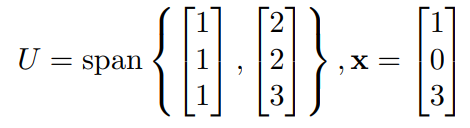
\includegraphics[width = \linewidth] {7a.png}
\end{figure}

a) Show that x $\notin$ U\\
\begin{figure}[H]
\centering
  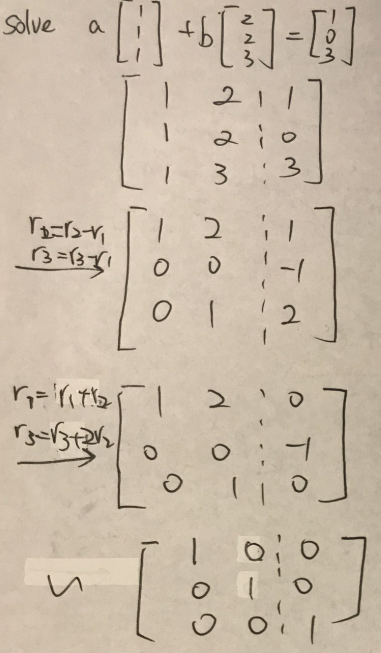
\includegraphics[width = 0.55\linewidth] {7b.png}
\end{figure}

In the last row is 0 $\cdot$ a + 0 $\cdot$ b = 1, which has no solutions. Therefore x $\notin$ U.\\

b) Determine the orthogonal projection $\pi_{U}$(x) of x onto U. Show that $\pi_U$(x) can be written as a linear combination of $[1, 1, 1]^T$ and $[2, 2, 3]^T$\\

As U = span{$[1, 1, 1]^T$,$[2,2,3]^T$}, x = $[1,0,3]^T$\\
The basis of Vector is:
\begin{equation*}
\begin{pmatrix}
1 & 2\\
1 & 2\\
1 & 3\\
\end{pmatrix}
\end{equation*}

Compute the $B^TB$ and the vector $B^Tx$:\\
\begin{gather}
B^TB = \begin{pmatrix}
1 & 1 & 1\\
2 & 2 & 3\\
\end{pmatrix} \cdot \begin{pmatrix}
1 & 2\\
1 & 2\\
1 & 3\\
\end{pmatrix} = \begin{pmatrix}
3 & 7\\
7 & 17\\
\end{pmatrix}
\end{gather}

\begin{gather}
B^Tx = \begin{pmatrix}
1 & 1 & 1\\
2 & 2 & 3\\
\end{pmatrix} \cdot \begin{pmatrix}
1\\
0\\
3\\
\end{pmatrix} = \begin{pmatrix}
4\\ 11
\end{pmatrix}
\end{gather}

Solve the normal equation $B^TB\lambda = B^Tx$ to get the value of $\lambda$:\\
\begin{gather}
\lambda = \begin{pmatrix}
-9/2 \\ 5/2
\end{pmatrix}
\end{gather}

\begin{gather}
\pi_U(x) = B \lambda =  \begin{pmatrix}
1/2\\1/2\\3
\end{pmatrix}
\end{gather}\\

\begin{equation}
\begin{pmatrix}
1 & 2 & 1/2 \\
1 & 2 & 1/2 \\
1 & 3 & 3 \\
\end{pmatrix}
\end{equation}
Minus the second row with the first row; minus the second row with the first row.
\begin{equation}
\begin{pmatrix}
1 & 2 & 1/2 \\
0 & 0 & 0 \\
0 & 1 & 5/2 \\
\end{pmatrix}
\end{equation}
Minus the first row with two times of third row.
\begin{equation}
\begin{pmatrix}
1 & 0 & -9/2\\
0 & 1 & 5/2\\
0 & 0 & 0\\
\end{pmatrix}
\end{equation}
$\pi_U(x)$ = $-\frac{9}{2} \cdot [1, 1, 1]^T + \frac{5}{2} \cdot [2,2,3]^T$\\
Therefore, $\pi_U$(x) can be written as a linear combination of $[1, 1, 1]^T$ and $[2, 2, 3]^T$\\

(c) Determine the distance d(x, U)\\
d(x,U) is the distance between the original vector and its projection onto U.
\begin{gather}
||x - \pi_U(x)|| = ||[-1/2,1/2,0]^T|| = \frac{\sqrt{2}}{2}
\end{gather}
\end{document}\\


